\subsection{Liquidity Simulation Environment\label{section:lse}}

As part of building Mosaic\cite{MosaicFinance} we wanted to understand the nature of liquidity and how its allocation and movement means for the design of the system.
%
To that end, Composable Labs\cite{IntroducingMedium} built a Liquidity Simulation Environment (LSE).\cite{IntroducingMediumb}

This software tool can simulate allocations of assets to vaults and assets moving around in the network.
%
It is modular and you can produce data in any form you want.
%
Currently, the LSE supports data generated from a truncated Gaussian, Geometric Brownian Motion (GBM), and data sampled from our 2021 September-October proof-of-concept (PoC) run.\cite{TestingMedium}

The strategy layer allows for any liquidity allocation and movement approach to be defined. For example "move liquidity from vault X to vault Y when conditions Z is true".
%
An objective - which can also be defined in the LSE - useful for searching for the best strategy could be to optimize the liquidity distribution among the vaults so that any transfer can be supported.

Fee models, how much and simply how, to charge moving assets can be defined as well. In fact, we used the PoC in conjuncion with the LSE to decide the best fee model to use in the context of available data up to that point.

The LSE is built as a state-machine iterating through the simulated transfers changing the states of the vaults. Replenishment events can be triggered - for example: the Arbitrum vault needs liquidity from the Mainnet vault.

The LSE is also continuously improving. As more transfer data is received this gives us a unique insight into how Mosaic is used and the LSE can help fine-tune our network to achieve an optimal user experience by having maximum availability.

\subsubsection{Simulating Data}

The LSE supports generating simulated transfer/usage data. We use this to model behavior of network usage and based on that make decisions on how to distribute liquidity.

We support generating data from a truncated Gaussian distribution. We sample a timeline and on that a set of hypothetical cross-chain cross-layer moves from this distribution with given mean and standard deviation.
%
We also support generating data from a Geometric Brownian Motion.
%
The moves or transactions $N_t$ (amount of \$) from one vault to another, at time $t$, following a GBM model, are described by the following stochastic differential equation (SDE)
\begin{equation}
\frac{d N_t}{dt} = \mu N_t + \sigma N_t\frac{dW_t}{dt}, 
\end{equation}
with $\mu$ being a drift term, $\sigma$ the volatility, both assumed to be constants and $W_t$ is a Brownian motion stochastic process. The analytical solution of the above SDE at time t, given initial condition $N_0$, is known to be 
\begin{equation}
\label{eq:gbm_solution}
N_t = N_0 \exp\left( (\mu - \sigma^2 / 2)t + \sigma W_t\right),
\end{equation}
which by definition is always strictly positive. A key property of the solution, important for our LSE use, is that the solution asymptotically goes to infinity when $\mu > \frac{1}{2}\sigma^2$, it goes to $0$ when $\mu < \frac{1}{2}$ and it fluctuates between zero and arbitrarily large values when $\mu = \frac{1}{2}\sigma^2$, therefore for most of our cases we will be using $\mu = \frac{1}{2}\sigma^2$. Fig. \ref{fig:gbm} shows two random simulation of eq. (\ref{eq:gbm_solution}) for the $N_0 = \$2000$, $\sigma=2$ and $N_0=\$1500$, $\sigma=1$ respectively. Note that the same initial and volatility values have also been used in our simulations below to simulate moves from Polygon to Arbitrum vaults and vice versa.
%
\begin{figure}[h]
    \centering
    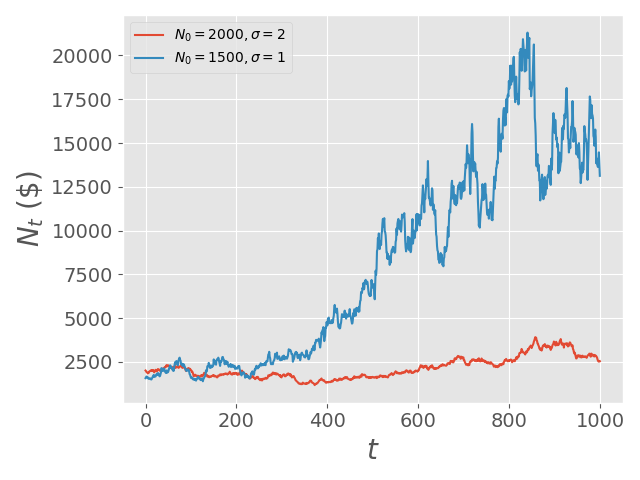
\includegraphics[width=0.5\textwidth]{images/gbms.png}
    \caption{Simulation of Geometric Brownian motion data in Composable's Liquidity Simulation Environment (LSE).}
    \label{fig:gbm}
\end{figure}
%

\subsubsection{Mosaic Fee Model}

One of the first use-cases of the LSE was deciding which fee model to use for Mosaic.
%
Fees are charged when funds are moved between networks. The question of which fee model to go with is key to a successful deployment.

Guided by Occam's razor\cite{WhatRazor} we picked a simple functional form following a linear fee model capped by a maximum fee amount ensuring that nobody, no matter how much they move across Mosaic, is charged more than a certain percent.

For most transfers, and for practically all retail transfers, users move along the linear part close to the origin. To ensure a safe network, we implemented a minimum fee as well distributing rewards to maintainers. Let $x$ denote the liquidity moved as percent of available liquidity in the origin vault. For example, if I move 10 ETH in a vault with 200 ETH $x=5$ (in units of \%). Let $y$ be the fee charged in percent. The Mosaic fee model is then determined by the two points $(x,y)=(0,0.25)$ and $(x,y)=(30,5)$.

The Mosaic PoC was run with this model and based on the data the two points were optimized to balance use and network safety (indirectly via rewards collected from fees).

\todo{Run different fee models. For each model:
Compute, based on PoC data (assuming those transfers), the fee revenue collected (APY). Want to strike balance b/w revenue and lowest fee possible too.}

\todo{plot fees from PoC on fee curve}
